\chapter{Introduction}

\section{Contexte}
L'Institut d'Automatisation Industrielle (iAi) dispose d'un démonstrateur de sustentation magnétique par attraction à quatre inducteurs. La régulation de position du véhicule a été étudiée et testée dans le cadre d'un précédent travail de bachelor. Bien que le résultat final n'ait pas donné entière satisfaction, plusieurs pistes ont été mises en avant pour améliorer la stabilité du système global.

La conception et le montage d'une nouvelle carte de commande équipée d'un DSP, ainsi que les circuits d'interfaçage des différents capteurs, ont été réalisés lors d'un précédent travail de bachelor.

Le but de ce projet consiste à finaliser le démonstrateur par la mise en œuvre et la programmation de la carte de commande pour la régulation des quatre inducteurs. Une interface utilisateur doit également être implémentée sur un site web embarqué, accessible via une liaison Wi-Fi.

\section{Historique du projet}

La maquette de démonstration a initialement été conçue en 1996 par Michel Zayadine \cite{Zayadine}, durant sa thèse de doctorat à l'EPFL en lien avec le projet Swissmetro. Son travail a consisté en la réalisation de la structure mécanique (chariot, quatre inducteurs et deux rails) ainsi qu'en l'élaboration de sa régulation. Le projet est néanmoins resté inutilisé pendant plusieurs années, avant que la maquette ne soit récupérée par l'institut iAi.

En 2018, Aymeric Dutruel \cite{Aymeric} a relancé le projet pour son travail de bachelor. Cette étude comprenait la réalisation des cartes de puissance pour chaque inducteur, le développement d'une carte d'interfaçage, l'intégration de capteurs laser de position ainsi qu'une première version des régulations de courant et de position pour un unique inducteur. Cependant, des problèmes de câblage ont limité la fiabilité des cartes, et le système nécessitait une assistance manuelle pour se stabiliser.

En 2019, Mattia Laucella \cite{Laucella} a fiabilisé les cartes de puissance et est parvenu à réaliser une régulation sur deux, puis quatre inducteurs. L'électronique a également été regroupée et fixée sur un support en bois afin que l'ensemble puisse être embarqué sur le chariot. Ce travail a permis d'obtenir une sustentation complète, bien qu'encore non optimale.

En 2022, Franck Yersin \cite{Yersin} a grandement fait évoluer le projet en développant une séquence de décollage. C'est également à partir de ces travaux qu'une interface utilisateur a été mise en place au moyen d'un Raspberry Pi couplé à un écran tactile. L'interface communiquait avec le DSP par liaison filaire et permettait d'observer le tracé de la position, tout en offrant la possibilité de modifier les paramètres de régulation.

En 2024, Christophe Isoz \cite{Isoz} a repris le projet afin de centraliser l'électronique sur une seule carte de contrôle. Le DSP a notamment été remplacé par une version plus moderne, un circuit de précharge pour les alimentations a été intégré, ainsi qu'un module de communication sans fil pour le Raspberry Pi (RaspBeeII). Malheureusement, ces travaux n'ont pas permis de remettre la maquette en lévitation en raison de défauts matériels et de temps de calcul trop longs.

En 2025, Thomas Freyche \cite{Freyche} a résolu les anomalies introduites précédemment dans la maquette. Son travail a consisté à corriger les erreurs de conception et à optimiser le code. Cette étape a permis, dans un premier temps, de réaliser une sustentation sur quatre inducteurs, mais à la suite d'une mauvaise calibration, la maquette n'a plus été apte à décoller.

\section{Les trains à sustentation magnétique}

\subsection{Histoire}

Les trains à sustentation magnétique (également appelés Maglev) utilisent les forces magnétiques pour se déplacer sans aucun contact avec les rails. Grâce à ce procédé, les résistances de roulement sont supprimées, ce qui permet d'atteindre des vitesses très élevées (le train japonais L0 a notamment atteint la vitesse de 603 km/h) \cite{Maglev}.

\begin{figure}[H]
    \centering
    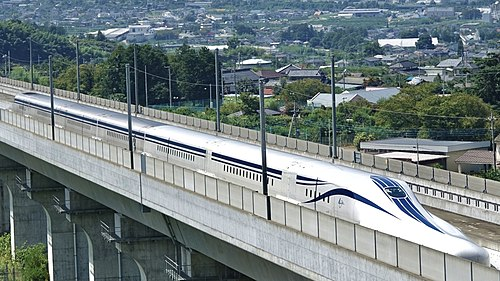
\includegraphics[width=0.53\linewidth]{Image/Chap.1/L0-950.jpg}
    \caption{Le train japonais L0 \cite{Maglev}}
\end{figure}

En Suisse, un projet de Maglev nommé Swissmetro a été développé dans le but de créer un train souterrain à l'intérieur de tunnels sous vide partiel. Le projet a été suspendu en 2009, et les droits associés ont ensuite été transférés à l'EPFL \cite{Swissmetro}.

\begin{figure}[H]
    \centering
    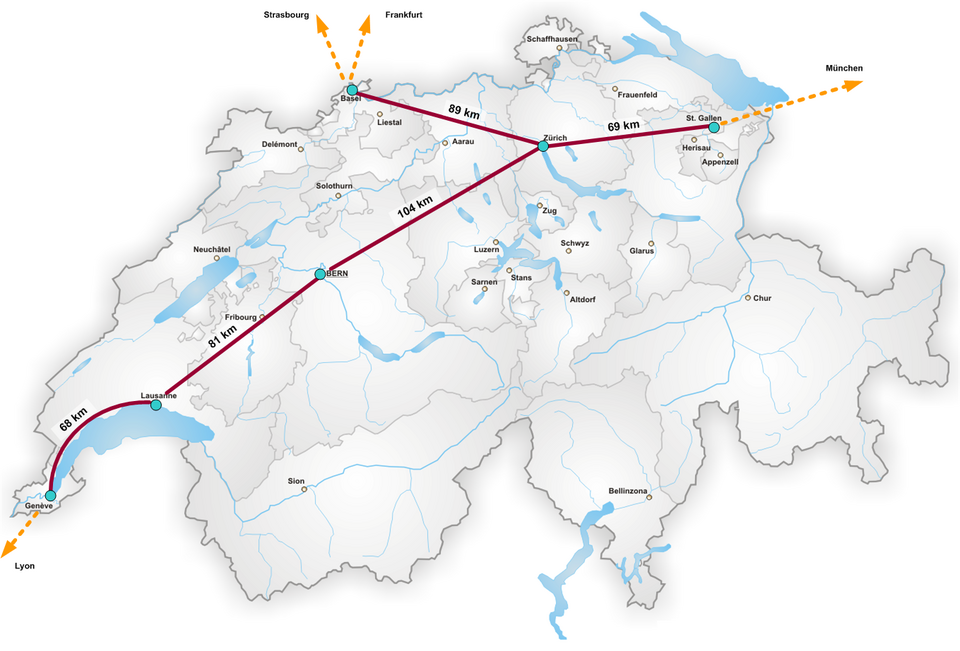
\includegraphics[width=0.6\linewidth]{Image/Chap.1/Swissmetro_Network_2005.png}
    \caption{Réseau du Swissmetro en 2005 \cite{Swissmetro}}
\end{figure}

\subsection{Principe}
Le démonstrateur utilise le principe de la sustentation magnétique par attraction (EMS, pour Electromagnetic Suspension). La lévitation repose sur trois aspects fondamentaux :

\begin{enumerate}
    \item La disposition mécanique : le chariot intègre des électroaimants (inducteurs) placés sous des rails ferromagnétiques fixes.
    \item La compensation de la gravité : le passage du courant dans les bobines génère un champ magnétique qui induit une force d'attraction vers le haut (en direction du rail), compensant ainsi le poids du chariot.
    \item La régulation active : l'exploitation des mesures des capteurs (courant et position) permet à la régulation d'empêcher un contact direct et violent entre les inducteurs et les rails.
\end{enumerate}

\begin{figure}[H]
    \centering
    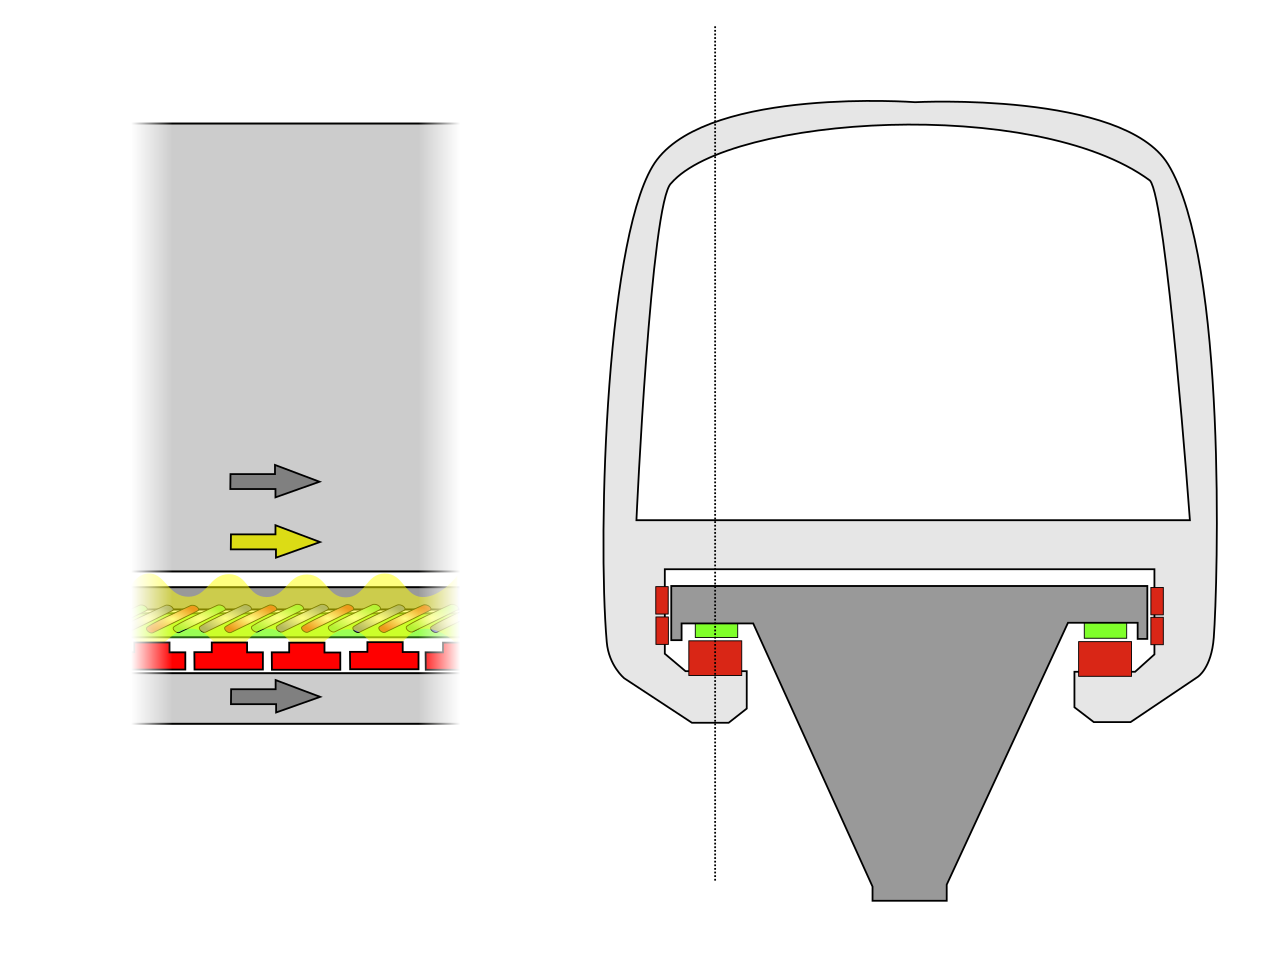
\includegraphics[width=0.6\linewidth]{Image/Chap.1/Magnetschwebebahn.png}
    \caption{Principe de l'EMS \cite{Swissmetro}}
\end{figure}

\section{Travaux à réaliser}
\red{A completer}
Les tâches à accomplir dans le cadre de ce projet sont les suivantes :

\begin{itemize}
    \item Identifier et corriger le dysfonctionnement présent dans le code principal.
    \item Finaliser l'interface utilisateur embarquée.
    \item Réaliser la synthèse d'un régulateur PID.
\end{itemize}

\section{Logiciels employés}
\begin{itemize}
    \item Code Composer Studio pour la programmation du DSP.
    \item Visual Studio Code pour la rédaction du rapport en \LaTeX.
    \item Excel pour la planification de Gantt, le traitement des mesures et la génération des graphiques.
    \item Draw.io pour la modélisation des schémas.
    \item Arduino IDE pour le développement du code de l'ESP32.
\end{itemize}

L'utilisation de Code Composer Studio requiert différentes installations et configurations préalables. Celles-ci sont détaillées dans la sous-section \ref{sec:MiseEnPlace}.

\section{Hypothèses de recherche}
\label{sec:Hypothese}

Plusieurs hypothèses ont été formulées concernant l'origine potentielle du problème de lévitation :

\begin{itemize}
    \item Les interruptions liées à la communication sans fil perturbent le bon déroulement de l'interruption dédiée à la régulation.
    \item Les contraintes temporelles ne sont plus respectées, ce qui nécessite une vérification de la durée d'exécution des tâches au sein de l'interruption.
    \item L'ajout récent d'une action intégrale engendre une instabilité du système.
    \item Une mauvaise calibration globale du système empêche le décollage.
    \item L'intégration de l'électronique embarquée a modifié la masse totale du système, faussant ainsi les paramètres de la régulation.
    \item Une erreur s'est glissée lors de la phase de synthèse des régulateurs.
    \item La condition de vérification à 99 \% perturbe le comportement de la machine d'état.
    \item La carte principale présente un défaut matériel.
    \item Les broches du DSP ne sont pas correctement reliées au reste de la carte principale.
\end{itemize}

\section{Usage de l'IA}
L'intelligence artificielle a été employée à des fins d'assistance pour les aspects suivants :
\begin{itemize}
    \item La rédaction (correction de la grammaire, de l'orthographe et amélioration de la structure du texte).
    \item La compréhension du code relatif au DSP et à l'ESP32.
    \item La structuration du code source et l'optimisation de sa lisibilité.
    \item Le soutien à l'analyse de la documentation des travaux précédents.
    \item Des interrogations générales concernant les principes théoriques appliqués.
\end{itemize}

En dehors de ces points, l'IA n'a pas été sollicitée pour d'autres tâches. L'outil principalement utilisé pour ce travail est Gemini. Une relecture systématique des retours a été effectuée afin de garantir la correspondance avec les attentes et la validité des informations.